% Standalone staged subsection; not inserted into the existing manuscript.
% The accompanying table/figure paths assume integration into the paper asset tree.
\subsection{Mini end-to-end training-step proxy}
\label{sec:phase4-training-proxy}

To examine whether sparse-index accumulation behavior remains visible within a
small backpropagation-style workload, Phase~4 embeds indexed lookup in a
synthetic computation comprising grouped mean pooling, a scalar linear prediction
head, mean squared error, and backward propagation. The three variants share
inputs, pooling, head, and loss: \texttt{embedding\_backward\_proxy} uses native
dense Embedding backward, whereas \texttt{index\_add\_proxy} and
\texttt{scatter\_add\_proxy} use custom autograd lookup nodes that allocate a dense
zero gradient and accumulate row gradients with the corresponding API.
This controlled proxy is not production training.

The \texttt{proxy\_step} scope measures a fresh lookup, pooling, prediction head,
loss, and gradients for the table, head, and bias. The
\texttt{accumulation\_region} scope separately replays backward through a retained
lookup graph with fixed upstream gradients, including dense gradient allocation,
zeroing, autograd dispatch, and accumulation. This second scope is a diagnostic
replay, not an exact decomposition of the proxy step; its latency must not be
subtracted from the total-step latency.

Each environment was evaluated with seeds 4001--4005 and 24 configurations per
seed, spanning 4,096 or 65,536 rows, 8,192 or 65,536 references, dimensions 32 or
128, and uniform, finite Zipf, or hotspot indices. Thus each environment contributes
120 seed--configuration observations, rather than 120 distinct shapes.
All ten runs completed, and all configurations and variants passed the recorded
validation against CPU float64 references with absolute tolerance $10^{-8}$ and
relative tolerance $10^{-4}$. Each scope used ten warmup iterations and forty
CUDA-event timing repetitions. A variant is a winner only if the runner-up median
divided by its median is strictly greater than 1.05; otherwise the observation is
a practical tie. This rule describes a practical margin, not statistical significance.

Table~\ref{tab:phase4-winner-counts} and
Figure~\ref{fig:phase4-winner-counts} summarize the results. On the local GTX1650Ti
stack, the index-add custom backward path won 83/120 proxy-step observations
(69.2\%) and 98/120 diagnostic-replay observations (81.7\%). Native Embedding won
ten observations in each scope, while 27 proxy-step and 12 replay observations
were ties. On the T4 stack, ties dominated: 95/120 (79.2\%) for the proxy step and
78/120 (65.0\%) for the replay. The remaining proxy-step observations favored
scatter-add (25/120); replay winners were mainly scatter-add (39/120), with three
index-add wins and no Embedding wins.

\begin{table}[tbp]
\centering\small
\caption{Phase 4 winners under the strictly greater than 5\% practical-margin rule. Each environment contributes 120 seed--configuration observations (24 configurations across five seeds). Region denotes a separate accumulation diagnostic replay.}
\label{tab:phase4-winner-counts}
\setlength{\tabcolsep}{3pt}
\resizebox{\linewidth}{!}{%
\begin{tabular}{llrrrrr}
\toprule
Environment & Scope & \texttt{index\_add} & \texttt{scatter\_add} & Embedding & Tie & Total \\
\midrule
GTX1650Ti & Proxy step & 83 & 0 & 10 & 27 & 120 \\
GTX1650Ti & Region replay & 98 & 0 & 10 & 12 & 120 \\
T4 & Proxy step & 0 & 25 & 0 & 95 & 120 \\
T4 & Region replay & 3 & 39 & 0 & 78 & 120 \\
\bottomrule
\end{tabular}
}%
\end{table}

\begin{table}[tbp]
\centering\small
\caption{Descriptive Phase 4 outcomes for the two measured environments. Differences cannot be attributed to GPU hardware alone because the software and host environments also differ.}
\label{tab:phase4-environment-comparison}
\setlength{\tabcolsep}{3pt}
\begin{tabularx}{\linewidth}{lXXX}
\toprule
Environment & Dominant proxy-step outcome & Dominant region-replay outcome & Interpretation \\
\midrule
GTX1650Ti & \texttt{index\_add}: 83/120 & \texttt{index\_add}: 98/120 & Custom index-add backward most often favored in this stack. \\
T4 & Practical ties: 95/120 & Practical ties: 78/120 & Resolved cases mainly favor \texttt{scatter\_add}; ties dominate both scopes. \\
\bottomrule
\end{tabularx}
\end{table}


\begin{figure}[tbp]
\centering
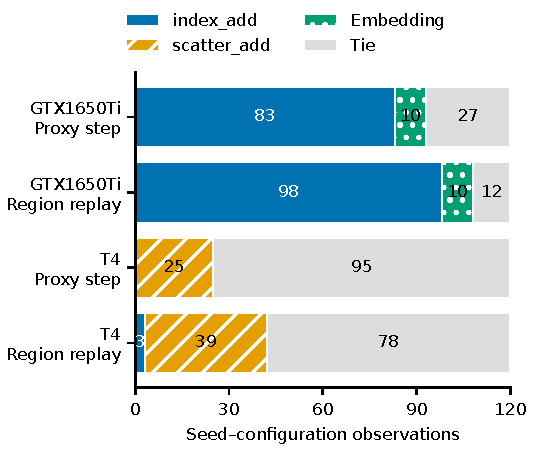
\includegraphics[width=\columnwidth]{figures/phase4_winner_counts_by_environment.pdf}
\caption{Phase~4 practical-margin winner counts across five seeds and 24
configurations per environment. Region replay is a separate diagnostic scope.
Ties are retained explicitly; counts do not establish statistical significance.}
\label{fig:phase4-winner-counts}
\end{figure}

The proxy does not identify a universal fastest API path. Instead, these results
reinforce the need to condition sparse-index accumulation conclusions on workload,
timing scope, software stack, and GPU environment. The GTX1650Ti environment used
PyTorch 2.13.0+cu126 and CUDA 12.6 on Windows; T4 used
PyTorch 2.11.0+cu130 with CUDA 13.0 on Linux; host thread settings also differed.
Consequently, the cross-environment contrast does not isolate hardware causality.
The local stack most often favored index-add, whereas the T4 stack was largely
unresolved by the practical-margin rule and its resolved cases mainly favored
scatter-add, especially in the replay. Isolated accumulation rankings should
therefore not be transferred mechanically to a training-step-like context without
measurement. These aggregates do not directly replicate Phase~2 rankings on a
matched set of configurations.

This proxy does not measure convergence, optimizer state, data loading,
distributed training, or production-scale model throughput. Parameters remain
fixed across repeated steps. The manual variants use custom autograd lookup nodes,
so the comparison is at the API/path level and includes dispatch and graph
overhead, rather than measuring pure kernel speed. Repeated timings and five
synthetic seeds do not establish performance across applications; timing
variability and the substantial T4 tie share further limit directional claims.
